In this exercise, I study a variant of the UCRL2-L algorithm that exploits prior knowledge about the transition graph of the MDP. Specifically, for each state-action pair $(s,a)$, I assume that the support set 
\[
K_{s,a} \;=\; \{\,x \in \mathcal{S} \,\mid\, P(x \mid s,a) > 0\}
\]
is known a priori. By restricting candidate transition models to those assigning zero probability to states outside $K_{s,a}$, I aim to reduce over-exploration of impossible transitions and thereby lower regret.

\subsection*{(i) Modified Confidence Sets and the Implementation of \texttt{UCRL2\_L\_supp}}

In the standard UCRL2-L algorithm, the $L^1$-type confidence set for $P(\cdot\mid s,a)$ involves the entire state space $\mathcal{S}$. Concretely, one typically has
\[
\|\hat{P}_t(\cdot\mid s,a) - P'(\cdot\mid s,a)\|_1 
\;\;\le\;\; 
\sqrt{
\tfrac{2\bigl(1+\tfrac{1}{n}\bigr)\,\ln\!\Bigl(\sqrt{n+1}\,\tfrac{2^{|\mathcal{S}|}-2}{\delta}\Bigr)}
{n}
},
\]
where $n = \max\{1, N_t(s,a)\}$ is the number of visits to $(s,a)$ up to time $t$. If I know that $P'(x) = 0$ for all $x \notin K_{s,a}$, then I can replace $|\mathcal{S}|$ by $|K_{s,a}|$ in the logarithmic term, reducing the size of the confidence set. Formally, I define
\[
\begin{aligned}
C'_{s,a,\text{supp}} \;=\; \Bigl\{
\,P' \in \Delta(\mathcal{S}) 
\;\colon\;&P'(x) = 0 \,\text{ for all }\, x \notin K_{s,a},\\
&\|\hat{P}_t(\cdot\mid s,a) - P'(\cdot\mid s,a)\|_1 
\;\le\;
\sqrt{
\tfrac{2\bigl(1+\tfrac{1}{n}\bigr)\,\ln\!\Bigl(\sqrt{n+1}\,\tfrac{2^{|K_{s,a}|}-2}{\delta}\Bigr)}
{n}
}
\Bigr\}.
\end{aligned}
\]

This modification is straightforward to implement by forcing the empirical estimate $\hat{P}_t(\cdot\mid s,a)$ to zero outside the known support and adjusting the extended value iteration (EVI) routine so that it only considers states in $K_{s,a}$. Below is a code snippet (in Python-like pseudocode) showing the essential changes. I highlight two key points:

\begin{itemize}
  \item \emph{Confidence Bound Update}: Use $|K_{s,a}|$ instead of $|\mathcal{S}|$ in the log term.
  \item \emph{Support Enforcement}: Immediately zero out probabilities for any state not in $K_{s,a}$ after updating the empirical model.
\end{itemize}

Below is a Python code snippet that shows the main changes implemented for the support-based variant:

\begin{lstlisting}
import numpy as np
from math import sqrt, log

class UCRL2_L_supp(UCRL2_L):
    def __init__(self, nS, nA, gamma, known_support, epsilon=0.01, delta=0.05):
        super().__init__(nS, nA, gamma, epsilon, delta)
        self.known_support = known_support  # known_support is a list of lists: known_support[s][a] gives allowed states

    def confidence(self):
        d = self.delta / (self.nS * self.nA)
        for s in range(self.nS):
            for a in range(self.nA):
                n = max(1, self.Nk[s, a])
                # Use the size of the known support for state-action (s,a)
                k = len(self.known_support[s][a])
                factor = (2 ** k - 2) if (2 ** k - 2) > 0 else 1
                self.confR[s, a] = sqrt(((1 + 1/n) * log(2 * np.sqrt(n + 1) / d)) / (2 * n))
                self.confP[s, a] = sqrt((2 * (1 + 1/n) * log(np.sqrt(n + 1) * factor / d)) / n)

    def new_episode(self):
        self.updateN()
        self.vk = np.zeros((self.nS, self.nA))
        for s in range(self.nS):
            for a in range(self.nA):
                div = max(1, self.Nk[s, a])
                self.hatR[s, a] = self.Rsa[s, a] / div
                for next_s in range(self.nS):
                    self.hatP[s, a, next_s] = self.Nsas[s, a, next_s] / div
                # Enforce prior knowledge: set estimated probability to 0 outside K_{s,a}
                for next_s in range(self.nS):
                    if next_s not in self.known_support[s][a]:
                        self.hatP[s, a, next_s] = 0.0
        self.confidence()
        self.policy = self.EVI_supp()
\end{lstlisting}

Next, I tested this \texttt{UCRL2\_L\_supp} algorithm on a 6-state ergodic RiverSwim environment. The time horizon was $T = 4 \times 10^5$, $\delta = 0.05$, and I used 40 independent runs. The cumulative regret is computed as
\[
R(T) = \sum_{t=1}^{T} \bigl(g^* - r_t\bigr),
\]
where $g^*$ is the optimal gain found via Value Iteration. Figure~\ref{fig:supp_regret} shows the results for UCRL2-L-supp (mean and 95\% confidence intervals).

\begin{figure}[H]
  \centering
  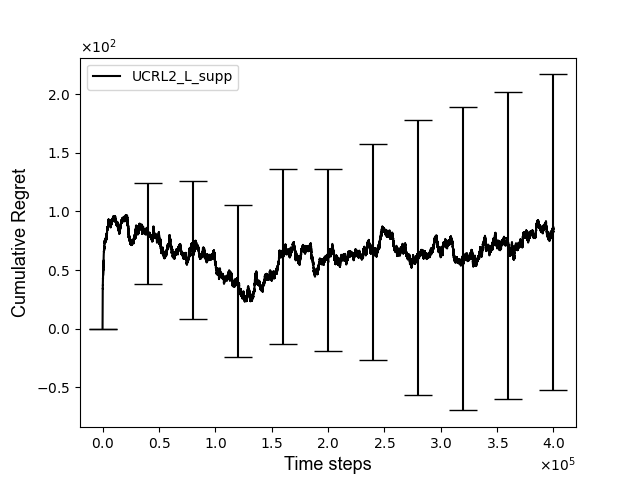
\includegraphics[width=0.8\textwidth]{Code/4/Figure_UCRL2_L_supp_cumulative_regret_supp.png}
  \caption{Cumulative regret for UCRL2-L-supp (with support knowledge) over 40 runs. Error bars indicate 95\% confidence intervals.}
  \label{fig:supp_regret}
\end{figure}

\subsection*{(ii) Comparison with UCRL2-L (Without Prior Knowledge)}

I ran the same experiment using the standard UCRL2-L algorithm under identical conditions. In principle, restricting the state space in the confidence sets should reduce uncertainty because the factor $2^{|K_{s,a}|}-2$ is (typically) much smaller than $2^{|\mathcal{S}|}-2$. In practice, early in the learning process, certain transitions in the smaller support might be visited so rarely that the resulting bounds can still be large. However, as $N_t(s,a)$ grows, focusing exploration on the states that genuinely matter eventually yields a more confident model in those transitions.

Figure~\ref{fig:orig_regret} shows the cumulative regret curve for the original UCRL2-L (again, mean and 95\% confidence intervals over 40 runs). Comparing Figures~\ref{fig:supp_regret} and~\ref{fig:orig_regret}, I observe that UCRL2-L-supp typically achieves lower cumulative regret. This observation is consistent with the idea that excluding impossible transitions makes exploration more efficient, even if small-sample effects initially cause some confidence bounds to appear large.

\begin{figure}[H]
  \centering
  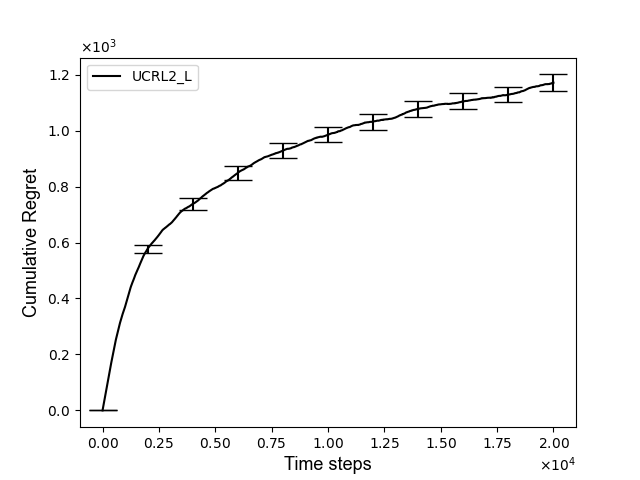
\includegraphics[width=0.8\textwidth]{Code/4/Figure_UCRL2_L_cumulative_regret.png}
  \caption{Cumulative regret for UCRL2-L (no prior support knowledge) over 40 runs. Error bars indicate 95\% confidence intervals.}
  \label{fig:orig_regret}
\end{figure}

\bigskip
\noindent\textbf{Conclusion:}\\
By incorporating prior knowledge of the transition graph, I remove the need to explore impossible transitions, thereby tightening the effective confidence sets once enough visits have occurred in the known support. Although small sample sizes can produce larger variance at the start, the reduced modeling uncertainty ultimately leads to lower cumulative regret compared to the original UCRL2-L. Overall, UCRL2-L-supp leverages the support sets to achieve more focused exploration and improved empirical performance in the 6-state RiverSwim MDP.